\documentclass[journal]{IEEEtran}
\IEEEoverridecommandlockouts

%%%%%%%%%%%%%%%%%%%%%%%%%%%%%%%%%%%%%%
%%%%%%%% PACCHETTI PRINCIPALI %%%%%%%%
%%%%%%%%%%%%%%%%%%%%%%%%%%%%%%%%%%%%%%
\usepackage{fancyhdr}
\usepackage{graphicx}
\usepackage[italian]{babel}
\usepackage[utf8]{inputenc}
\usepackage{color}
\usepackage{hyperref}
\usepackage{wrapfig}
\usepackage{array}
\usepackage{multirow}
\usepackage{adjustbox}
\usepackage{nccmath}
\usepackage{subfigure}
\usepackage{amsfonts,latexsym}
\usepackage{enumerate}
\usepackage{booktabs}
\usepackage{float}
\usepackage{threeparttable}
\usepackage{array,colortbl}
\usepackage{ifpdf}
\usepackage{rotating}
\usepackage{cite}
\usepackage{stfloats}
\usepackage{url}
\usepackage{listings}
\usepackage{soul}

%%%%%%%%%%%%%%%%%%%%%%%%%%%%%%%%%%%%
%%% CREA E SCRIVI ALCUNI COMANDI %%%
%%%%%%%%%%%%%%%%%%%%%%%%%%%%%%%%%%%%
\newcolumntype{P}[1]{>{\centering\arraybackslash}p{#1}}  %% Viene creato un nuovo tipo di colonna denominata P.

% correggere la sillabazione errata qui
\hyphenation{op-tical net-works semi-conduc-tor} %% Con questo comando si specifica come separare correttamente le sillabe nel caso in cui una parola si trovi in due diverse righe di testo

\graphicspath{ {img/} }  %%Percorso dove si trovano le immagini, se è vuoto indica che le immagini sono all'interno della stessa cartella che contiene il file .tex


%%%%%%%%%%%%%%%%%%%%%%%%%%%%%%%%%%%%%%%%%%%%%%%%
%%% INTESTAZIONE DELLE PAGINE TIPO UNICAFAM %%%%
%%%%%%%%%%%%%%%%%%%%%%%%%%%%%%%%%%%%%%%%%%%%%%%%
\newcommand{\MYhead}{\smash{\scriptsize
\hfil\parbox[t][\height][t]{\textwidth}{\centering
\begin{picture}(0,0) \put(-30,-13){
\includegraphics[width=30mm]{logoUnisalento.jpg}} \end{picture} \hspace{6.4cm}
INGEGNERIA INFORMATICA \\
\hspace{5.2cm} DIPARTIMENTO DI INGEGNERIA DELL'INNOVAZIONE \hspace{3cm} \\
\underline{\hspace{ \textwidth}}}\hfil\hbox{}}}
\makeatletter

% normal pages
\def\ps@headings{%
\def\@oddhead{\MYhead}%
\def\@evenhead{\MYhead}}%

% title page
\def\ps@IEEEtitlepagestyle{%
\def\@oddhead{\MYhead}%
\def\@evenhead{\MYhead}}%
\makeatother

% make changes take effect
\pagestyle{headings}

% adjust as needed
\addtolength{\footskip}{0\baselineskip}
\addtolength{\textheight}{-1\baselineskip}

%define colors for code language
\definecolor{codegreen}{rgb}{0,0.7,0.3}
\definecolor{codegray}{rgb}{0,0,0}
\definecolor{codepurple}{rgb}{0.58,0,0.82}
\definecolor{backcolour}{rgb}{0.95,0.95,0.95}
\definecolor{keywordcolor}{rgb}{0.8,0.3,0}

\lstdefinestyle{mystyle}{
    backgroundcolor=\color{backcolour},   
    commentstyle=\color{codegreen},
    keywordstyle=\color{keywordcolor},
    numberstyle=\tiny\color{codegray},
    stringstyle=\color{codepurple},
    basicstyle=\ttfamily\footnotesize,
    breakatwhitespace=false,         
    breaklines=true,                 
    captionpos=b,                    
    keepspaces=true,                 
    numbers=left,                    
    numbersep=5pt,                  
    showspaces=false,                
    showstringspaces=false,
    showtabs=false,                  
    tabsize=4
}

\lstset{style=mystyle}



%%%%%%%%%%%%%%%%%%%%%%%%%%%%%%%%
%%%%% INIZIO DEL DOCUMENTO %%%%%
%%%%%%%%%%%%%%%%%%%%%%%%%%%%%%%%
\begin{document}



%%%%%%%%%%%%%%%%%%%%%%%%%%%%
%%% TITOLO DEL DOCUMENTO %%%
%%%%%%%%%%%%%%%%%%%%%%%%%%%%
\title{Gestione dei Big Data}



%%%%%%%%%%%%%%%%%%%%%%%%%%
%%%%%%%%% AUTORE %%%%%%%%%
%%%%%%%%%%%%%%%%%%%%%%%%%%
\author{Matteo Aprile\\
				Professore: Marco Zappatore, Antonella Longo\\
        }
        
%scrive il titolo
\maketitle

%scrive l'indice
\tableofcontents
\underline{\hspace{ 80 mm }}



%%%%%%%%%%%%%%%%%%%%%%%%%%%%%
%%% SEZIONI DEL DOCUMENTO %%%
%%%%%%%%%%%%%%%%%%%%%%%%%%%%%

\section{Libri di testo consigliati}
\itemize{}
	\item Advanced Programming in the Unix Environment, 3th ed, Stevens, Rago
	\item TCP/IP 1, Stevens (facoltativo)
	\item Unix Networking Programming the Socket Networking API, Stevens
	\item The Linux Programing Interface, Kerrisk
	\item manset
	\item Gapil Guida alla Programmazione in Linux, Simone Piccardi
\newpage
\section{Databases - 28.09.22}

% Definizioni di base
\subsection{Definizioni di base}

Le definizioni di base da sapere sono:
\begin{itemize}
	\item \hl{dato}: \textbf{insieme di fatti conosciuti, registrati e con un significato}. È detto dato grezzo visto che si suppone che andrò ad elaborarlo, questo dato \textbf{sara' poi archiviato}, sarà un \textbf{fatto conosciuto} cioè avremo:
		\begin{itemize}
			\item \textbf{eventi con un significato} per un dato tipologia di utenti 
			\item sorgente che \textbf{produce i dati} con una cerca velocità
		\end{itemize}
	
	\item \hl{DataBase}: \textbf{raccolta di dati altamente organizzati, intercorrelati e strutturati}. È una struttura con dei collegamenti strutturati tra i dati

	\item \hl{DBMS Data Base Managment System}: insieme di \textbf{programmi per accedere ai dati e farci delle operazioni} di 4 tipi: creazione, recupero, aggiornamento e cancellazione, ciclo \textbf{CRUD}. Ne favorisce anche il mantenimento.

	\item \hl{mini-world}: \textbf{parte del mondo reale alla quale si riferiscono i dati presi} andando a \textbf{limitare la modellazione} in un numero n di concetti

	\item \hl{DataBase System}: insieme di DBMS con i dati
	
	\item \hl{astrazione}: \textbf{separare i dati dai collegamenti tra le entità per disporle in un modello} senza che esso si occupi di come salvare i dati
	
	\item \hl{modello concettuale}: formato da entità e relaizoni
	
	\item \hl{modello fisico}: definizione dei tipi dato e dove sono \textbf{conservati}
	
	\item \hl{controllo della concorrenza}: garantire che tutte le transazioni sono \textbf{correttamente eseguite}
	
	\item \hl{recovery}: se la transazione è stata eseguita è stata conservata nel database
\end{itemize}


% Tipologie di DB
\subsection{Tipologie di DB}

Esistono molti tipi di DB:

\begin{itemize}
	\item numerici o testuali
	\item multimediali
	\item Geographic Information Systems (GIS)
	\item Data Warehouses
\end{itemize}


% Ciclo di vita del DB
\subsection{Ciclo di vita del DB}

È opportuno vedere un \hl{concetto di base dei dati}, cioè il loro ciclo di vita. Il più semplice è:

\begin{enumerate}
	\item \textbf{acquisizione} (scattered data)
	\item \textbf{aggregazione} (integrated data)
	\item \textbf{analisi} (knowledge)
	\item finisce in un \textbf{applicazione} che genera dei "log data" che saranno poi acquisiti come scattered data
\end{enumerate}

Da un \hl{punto di vista computazionale} queste fasi si devono prendere in un altro modo:

\begin{enumerate}
	\item storage dei data
	\item formattazione e pulizia
	\item capire cosa dicono i dati
	\item[?)] se non mi bastano i dati che ho posso integrare dei dati
\end{enumerate}


% Livelli di un DB
\subsection{Livelli di un DB}

Quando si ha un DB abbiamo 3 livelli da considerare

\begin{enumerate}
	\item \hl{fisico}: dove sono \textbf{salvati i dati}
	\item \hl{logico}: indica come i dati sono \textbf{collegati tra loro}
	\item \hl{view}: \textbf{rappresentazione} che sarà diversa per ogni tipo di utente
\end{enumerate}


% DBMS Data Base Managment System
\subsection{Data Base Managment System}

Un DBMS offre l'opportunità di:

\begin{itemize}
	\item \textbf{salvataggio} dei dati
	\item \textbf{definizione} modelli dati
	\item \textbf{manipolazione} dei dati
	\item \textbf{processare} e condividere i dati
\end{itemize}

Per quanto riguarda l'\hl{interazione con i DB} avremo 2 strumenti:

\begin{itemize}
	\item \hl{query}: accede a parti differenti di dati e formula una richiesta
	\item \hl{transazioni}: legge dei dati ed aggiorna alcuni valori, salvandoli nel DB
\end{itemize}


% Mini-world
\subsection{Mini-world}

Avremo bisogno di \hl{identificare delle entita'}, cioè i \textbf{concetti di base} che rappresentano una parte delle cose che inseriremo nel DB relazionale. Poi andremo a \hl{connettere tra loro le entita'}, dette relazioni (\hl{relationships}) (ER), \hl{ne derivano delle tabelle dette relation}.

Il tutto \hl{da derivare dai requisiti} e non dall'esperienza personale.

Le tabelle create dalle entità conterranno i dati che ho a disposizione. Saranno divisi in:

\begin{itemize}
	\item righe (record)
	\item colonne (attributi)
	\item celle (dati grezzi)
\end{itemize}


Si verrà quindi a creare un \hl{catalogo} con vincoli, tipo di dati e la relazione di appartenenza degli attributi.

\newpage
\section{Database System Concepts and Architecture - 28.09.22}

% Definizioni sui modelli
\subsection{Definizioni sui modelli}

Le definizioni di base da sapere sono:

\begin{itemize}
	\item \hl{Data Model}: insieme di \textbf{concetti che descrivono struttura, operazioni e vincoli} applicati al DB
	
	\item \hl{Data Model Structure and Constraints}: abbiamo dei \textbf{costrutti che definiscono come collegare gli elementi} definiti da: entità, record e tabella

	\item \hl{Data Model Operation}: di base (\textbf{CRUD}) o definite dall'utente

	\item \hl{modello dal concettuale}: di \textbf{alto livello} e semantico
	
	\item \hl{modello fisico}: di basso livello, definisce \textbf{come i dati sono salvati}
	
	\item \hl{modello implementativo}: usati nel DBMS 
	
	\item \hl{modello autodescrivente}: basati su XML 

\end{itemize}


% Definizioni fondamentali
\subsection{Definizioni fondamentali}

\begin{itemize}
	\item \hl{DataBase schema}: descrizione del database in termini di struttura, tipo dati e vincoli
	
	\item \hl{schema diagram}: \textbf{visione rappresentativa} del DB schema
	
	
\begin{figure}[H]
\centering
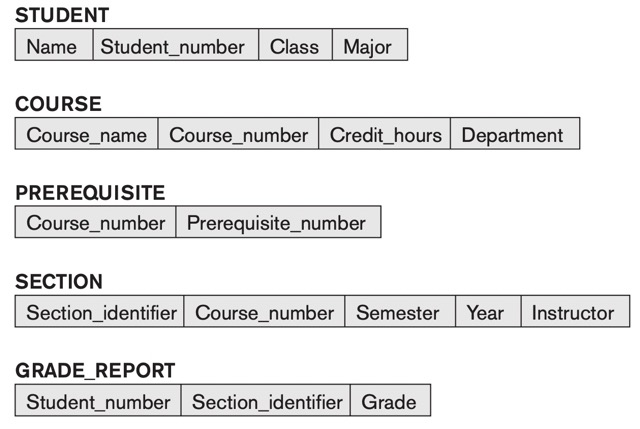
\includegraphics[scale=0.4]{schcon.jpeg}
\caption{Schema diagram} 
\label{schcon}
\end{figure}
	
	
	\item \hl{schema construct}: insieme tra \textbf{schema e dati} dei DB


	\item \hl{database state}: \textbf{snapshot} in istante t del DB, si definisce quindi ai suoi contenuti
	
	\item \hl{valid state}: si definisce funzionante se il suo contenuto \textbf{soddisfa i vincoli} per quello schema
	
	\item \hl{data dictioraty}: insieme per salvare schema e altre info 
\end{itemize}


% Schema
\subsection{Schema}

Possiamo avere 3 \hl{livelli di schema}:

\begin{enumerate}
	\item \textbf{interno (fisico)}: come i dati devono essere salvati e come posso accederci
	\item \textbf{concettuale}
	\item \textbf{esterno}: per descrivere le view dell'utente
\end{enumerate}


\hl{Per passare da uno schema ad un altro} ho bisogno di un \hl{mapping} per capire a cosa corrisponde un elemento. Avremo:

\begin{itemize}
	\item \hl{logic data independence}: se voglio \textbf{cambiare lo schema concettuale} senza cambiare quello fisico
	\item \hl{physical}: devo \textbf{cambiare lo schema fisico} senza cambiare quello concettuale
\end{itemize}


% Tipologie di DBMS
\subsection{Tipologie di DBMS}

Possiamo avere più tipologie di DBMS:

\begin{itemize}
	\item \hl{centralized}: dove abbiamo tutta l'\textbf{elaborazione su un unico nodo}
	\item \hl{2-tier}: si specializza in termini di server per ogni blocco di funzionalità che devo offrire
	\item \hl{cliets}: per far accedere gli utenti
	\item \hl{DBMS server}: per eseguiire query e transazioni tramite API
\end{itemize}


\newpage
\section{Data Modeling Using the Entity–Relationship (ER) Model - 28.09.22}


% Entity-Relationship (ER)
\subsection{Entity-Relationship (ER)}

Partendo dal mini-world serve \hl{capire i requisiti utili}. Bisognerà far gestire, all'applicazione, alcuni dati per poi visualizzarli (requisiti relazionali).

La procedura sarà:

\begin{enumerate}
	\item acquisizione dei data requirements
	\item conversione in un modello concettuale
	\item applicazione dell'algoritmo di mapping
	\item DBMS si occupa di physics design ed internal schema
\end{enumerate}

in parallelo avremo la \hl{gestione delle transazioni} del mini-world estraendo i functional requirements per effettuare una functional analysis che genera delle transazioni ad alto livello.


Per la scelta degli elementi avremo:

\begin{itemize}
	\item \hl{entita' (sostantivi)}: \textbf{oggetti o cose specifiche} presenti nel mini-world che bisogna rappresentare

	\item \hl{relazioni (verbi)}: \textbf{collegano le entita'}. Il \textbf{grado di tipo} della relazione è il \textbf{numero di partecipanti a quella relazione}, identificando quante volte la relazione viene percorsa.
		
		Può:
		\begin{itemize}
			\item essere \textbf{ricorsiva} se si riferisce ad una stessa entità
			\item avere un suo attributo definito dall'azione che sta compiendo
		
		\end{itemize}
		
		

	
	\item \hl{attributi (proprieta')}: \textbf{descrittori} per ogni entità
	
	\item \hl{record}: \textbf{insieme degli attributi} che si danno ad un entità
	
	\item \hl{dato singolo}: ha un unico valore
	
	\item \hl{dato composto}: dati da un \textbf{insieme di più descrittori}, notazione: ...(... , ...)
	
	\item \hl{dato multivalore}: attributi che hanno \textbf{n-uple di valori}, notazione: {...}
	
	\item \hl{attributo chiave}: \textbf{identificare univocamente tutti i record}. Si può usare anche un'unione tra attributo chiave e un altro attributo
	
	\item \hl{entita' debole}: entità che \textbf{da sola non può esistere}, quindi dipende da un entità più forte. Le sue relationship saranno deboli anche esse. Questa entità \textbf{non ha un attributo chiave} ma ha almeno un \textbf{attributo in comune con l'entità forte}.
	
	\item \hl{vincoli}: ci sono dei concetti che fungano da vincoli
	
		\begin{itemize}
			\item \textbf{impliciti}: come è definito il modello dati (es: non posso avere una lista come valore di un attiributo, allora userò n colonne per quanti sono i possibili numeri di telefono)
			
			\item \textbf{espliciti}: aggiunti dal modellista (es: cardinalità min max)
			
			\item \textbf{semantici}: vincoli aggiunti dal programmatore che farà l'applicativo sul quale si base il nostro db (es: la psw deve avere un tot di caratteri e non altri)
		\end{itemize}
	
\end{itemize}

Piccoli \hl{accorgimenti da avere}:

\begin{itemize}
	\item scritto da \textbf{sx a dx} e dall'altro verso il basso
	
	\item nomi delle \textbf{entita' al singolare}
	
	\item \textbf{verbi alla terza persona} e attivi o passi per capire da che parte si deve leggere la relazione
	
	\item per la \textbf{carcinalita'} mi chiedo per un solo elemento quante entità puotrà avere dell'altro a cui è relazionato. Può essere rappresentata tramite:
	
		\begin{itemize}
			\item \textbf{vincoli di dipendenza esistenziale}: 1:1, 1:N, M:N dove bisogna mettere la cardinalità nel lato opposto
			\item \textbf{min max}: dico che posso avere da un min a un max di record che percorrono la relazione dando in vincolo di intervallo (sarà di aiuto a chi farà il database quando dovrà gestire un warning)
		\end{itemize}
	
	 
\end{itemize}


I database NoSQL saranno esenti da una modellazione così pesante.


Potremmo incombere in \hl{relazioni di livello piu' alto} nel caso in cui ci trovassimo a descrivere relazioni con complessità alto. In gnerale \hl{si cerca di evitare e di farlo con relazioni binarie} per evitare complicazioni nell'implementazione.


\begin{figure}[H]
\centering
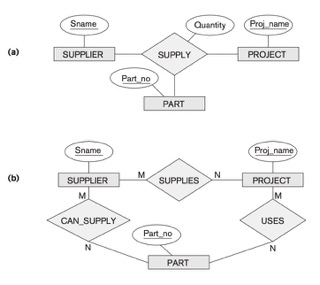
\includegraphics[scale=0.7]{relazlivalt.jpeg}
\caption{Relazione di livello alto} 
\label{relazlivalt}
\end{figure}

\newpage
\section{The Enhanced Entity–Relationship (EER) Model - 04.10.22}


% Superclassi e sottoclassi
\subsection{Superclassi e sottoclassi}

L'idea è di andare a creare una \hl{gerarchia}:


\begin{figure}[H]
\centering
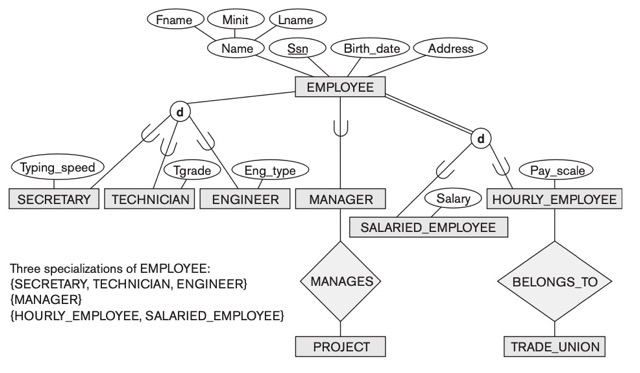
\includegraphics[scale=0.4]{gerardisg.jpeg}
\caption{Gerarchia con disjoint} 
\label{gerardisg}
\end{figure}


Per modellarlo mi chiedo quali siano le \hl{caratteristiche che hanno in comune alcune entita'}, allora tutti gli \hl{attributi in comune vanno nella superclasse}. \hl{Ogni entita' DEVE avere i suoi attributi specifici} ma non ho un attributo chiave dato che viene preso dalla superclasse.


% Graficazione superclassi e sottoclassi
\subsection{Graficazione superclassi e sottoclassi}

La graficazione avrà per:

\begin{itemize}
	\item \hl{specializzazione diretta}: si ha un segmento 
	\item \hl{gerarchia (IS-A)}: si ha un segmento con un nodo con:
		
		\begin{itemize}
			\item \textbf{d -$>$ disjoint}: NON POSSO avere un'entità che è contemporaneamente due o più sottoentità (\textbf{solo una})
			\item \textbf{o -$>$ overlap}: posso avere un'entità che è contemporaneamente due o più sottoentità (\textbf{almeno una})
			\item \textbf{U - $>$ union}: \textbf{raggruppa} entità di tipo diverso
		\end{itemize}
		
		le quali potranno avere \hl{partecipazioni totali o parziali} che indicano se la superclasse deve o meno scegliere tra le sottoclassi.
		
\end{itemize}


\begin{figure}[H]
\centering
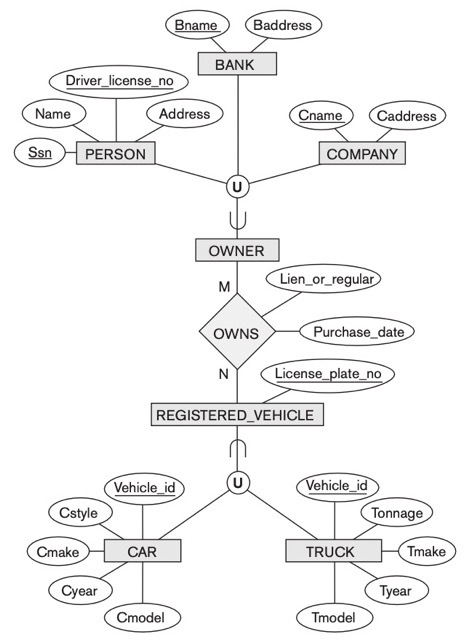
\includegraphics[scale=0.4]{union.jpeg}
\caption{Gerarchia con disjoint} 
\label{gerardisg}
\end{figure}



Il motivo della modellazione è la presenza di alcune \hl{fasi per i sistemi di gestione delle informazioni}:

\begin{itemize}
	\item studio di fattibilità
	\item analisi dei requisiti
	\item modellazione e design
	\item prototipo (ciclico)
	\item implementazione
\end{itemize}


Per i relazionali le fasi sono:

\begin{itemize}
	\item application requirements
	\item modello concettuale
	\item modello logico
	\item modello fisico
\end{itemize}


% Notazioni
\subsection{Notazioni}

Nella creazione del modello usiamo la notazione:


\begin{figure}[H]
\centering
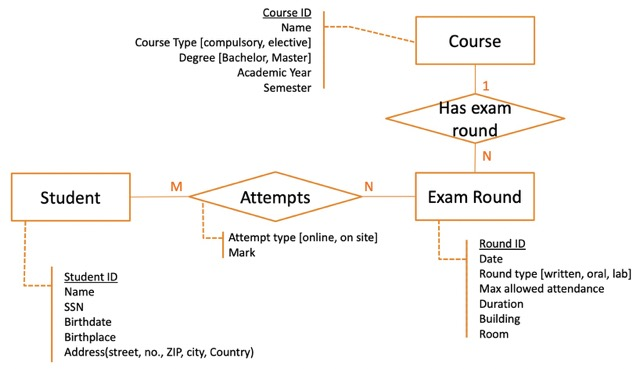
\includegraphics[scale=0.4]{notaz.jpeg}
\caption{Notazione dei diagrammi ER} 
\label{notaz}
\end{figure}


se un \hl{attributo puo' avere solo un numero finito di valori} si usa: $$...[... , ...]$$


Se ho bisogno di \hl{sostituire una connessione logica con un entita'} la chiamo: \hl{reificazione}. La si usa se si ha la \hl{necessita' di creare un entita' sulla quale si baseranno altre relationship}. Se sbaglio il verso delle relationship metto una freccia.


\begin{figure}[H]
\centering
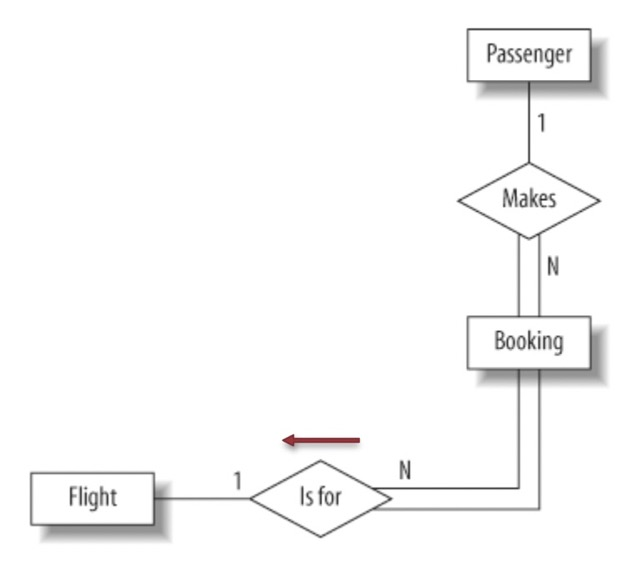
\includegraphics[scale=0.3]{reifi.jpeg}
\caption{Reificazione ed orientamento della relationship} 
\label{reifi}
\end{figure}


conviene usare delle relation con un nome univoco.


% Terminologia
\subsection{Terminologia}


\begin{table}[h!]
	\begin{center}
		\begin{tabular}{|c | c|} 
			\hline
			termine informale & termine formale \\ [0.5ex]
			\hline
 			table & relation \\
			column header & attribute \\
			all possible column values & domain \\
			row & tuple "<...>" \\\hline
			table definition & schema of a relation \\
			populated table & state of the relation \\
			\hline
		\end{tabular}
	\end{center}
	\caption{Tabella delle ore di lavoro}
	\label{taborelav}
\end{table}


\begin{figure}[H]
\centering
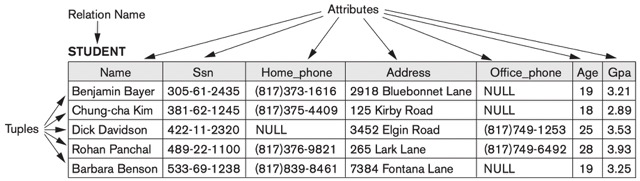
\includegraphics[scale=0.4]{termformtab.jpeg}
\caption{termini formali per le tabelle} 
\label{termformtab}
\end{figure}


\newpage
\section{Basic SQL}


SQL è un linguaggio che consente di accedere al db in varie modalità ed \hl{ha la funzione di creare e gestire i db}.


% Statement - SELECT
\subsection{Statement - SELECT}

Usato per \hl{recuperare informazioni dal db}. la sua struttura ha 3 clausole (claude):

\begin{lstlisting}
SELECT <attribute list>
FROM <table list>
[ WHERE <condition> ]
[ ORDER BY <attribute list> ];
\end{lstlisting}


Molto utile usare gli \hl{alias (AS)} per:

\begin{itemize}
	\item andare a \textbf{definire i campi che ci serviranno in modo da dividere gli attributi di una tabella con quelli di un altra}
	
	\item \textbf{accedere ad una stessa tabella ma con 2 alias diversi} perchè per esempio uno rappresenta l'impiegato e l'altro il supervisore
	
	\item \textbf{rinominare gli attributi}:

\begin{lstlisting}
EMPLOYEE AS E(Fn, Mi, ...)
\end{lstlisting}


\end{itemize}


\hl{Keyword} da poter usare:

\begin{itemize}
	\item \textbf{DISTINCT}: restituisce solo valori distinti (diversi) nel set di risultati
\end{itemize}


% Statement - WHERE
\subsection{Statement - WHERE}

\hl{Esprime una condizione}, se manca è possibile fare il prodotto cartesiano se si usa:

\begin{lstlisting}
SELECT Ssn, Dname
FROM EMPLOYEE, DEPARTMENT
\end{lstlisting}

Si possono usare delle condizioni di tipo:

\begin{itemize}
	\item numerico:

\begin{lstlisting}
WHERE Dno = 5
\end{lstlisting}

	\item pattern matching tra stringhe:

\begin{lstlisting}
WHERE Ssn LIKE "yes"
\end{lstlisting}
	
		se non è un occorrenza esatta usiamo:

			\begin{itemize}
				\item \textbf{\%}: indica una qualsiasi sottostringa
				\item \textbf{\_}: indica un solo carattere in una specifica posizione
			\end{itemize}

\end{itemize}


% Statement - ORDER BY
\subsection{Statement - ORDER BY}

Per ordinare i risultati con DESC o ASC.





\end{document}
%%%%%%%%%%%%%%%%%%%%%%%%%%%%%%%%
%%%%%% FINE DEL DOCUMENTO %%%%%%
%%%%%%%%%%%%%%%%%%%%%%%%%%%%%%%%




